\section{Derivation of Segway Transfer Functions}
In this section, the model expressions derived in previous sections are verified, linearized and combined into transfer functions. From these transfer functions, the controllers will be designed to allow the segway to balance in an upright position. In this section, the models are viewed and linked as illustrated in \autoref{fig:modelOverallLin}.
\begin{figure}[H]
\centering
\begin{tikzpicture}[auto, node distance=3.5cm,>=latex']
    % We start by placing the blocks
    \node [input, name=input] {};

    % Once the nodes are placed, connecting them is easy. 
	\draw[thick,dashed, fill=black!10, align=center] ($(input.north west)+(15.5,-1)$) rectangle ($(input.north west)+(0.6,2.75)$);
	\draw[thick,dashed, fill=black!30, align=center] ($(input.north west)+(10.75,-0.8)$) rectangle ($(input.north west)+(1.5,1.75)$);
	 \node [align=center] at ($(input.north west)+(8,2.25)$) {\textbf{Plant, }$\mathbf{ \, \, \, G}$};
	 \node [align=center] at ($(input.north west)+(6,1.25)$) {{Motors and Wheels Model}};
	
	\node [blockbig, right of=input, align = center] (motor) {Motor \\ and Wheel};
	\node [blockbig, right of=motor, align = center, node distance=4.5cm] (Cart) {Cart \\ Movement};
    \node [blockbig, right of=Cart, align = center, node distance=4.5cm] (pendulum) {Inverted \\ Pendulum};

   \node [output, right of=pendulum, node distance=3.5cm] (output) {};

	
    \draw [->] (input) -- node {$V_a$} (motor);
    \draw [->] (4.75,0.2) -- node {$\tau_a$} (6.75,0.2);
    \draw [->] (9.25,0.2) -- node {$\theta_w$} (11.25,0.2);
    \draw [->] (11.25,-0.2) -- node {$F_L$} (9.25,-0.2);
   % \draw [->] (9.75,-0.2) -| node {} (3.75,-0.2);
    \draw [->] (pendulum) -- node {$\theta_p$} (output);
\end{tikzpicture}
\caption{Block diagram of the plant, also known as system model.}
\label{fig:modelOverallLin}
\end{figure}
Note that the models are linked differently than previously shown in \autoref{fig:modelOverall}, since the cart movement is made part of the motor and wheel model, instead of being part of the inverted pendulum model. This is because it is not possible to measure the torque $\tau_a$, while the wheel angle, $\theta_w$, can be measured by the encoders. Thus, it will be possible to derive a transfer function for the motors and wheels model. The same applies for the inverted pendulum model, where it will be possible to derive and verify a transfer function based on an input being the wheel angle, $\theta_w$, instead of the torque $\tau_a$.
\subsection{Verification of Models}
The three model expressions that have been derived in the previous sections are \autoref{eq:MotorFinal}, \ref{eq:model_pen33} and \ref{eq:inertia1}. For repetition, these are shown below.
\begin{align}
\tau_a(t) = \frac{1}{N_{ms} N_{sw}}\Big(\frac{k_t}{R_a} \big( V_a(t)& - k_e \dot\theta_m(t) \big) - \ddot\theta_m(t)J_{T} - \dot\theta_m(t)B_{T}\Big)
\label{eq:model3}\\
m_c \cdot \ddot x_c(t) = F_F(V_a(t)) - m_p\Big(\ddot x_c(t)& + l \cdot \sin(\theta_p(t))\cdot \dot\theta_p^2(t) - l \cdot \cos(\theta_p(t))\cdot \ddot\theta_p(t)\Big)\label{eq:model2}\\
(J_p+m_p\cdot l^2)\cdot \ddot \theta_p(t) = m_p \cdot l \cdot &\left( \sin(\theta_p(t)) \cdot g+\cdot \cos(\theta_p(t)) \cdot \ddot x_c(t) \right) \label{eq:model1}
\end{align}

If no slip is assumed in the gearing and between the wheels and the ground, then $\dot \theta_m(t)$ and $\ddot \theta_m(t)$ can be replaced with $N_{ms}N_{sw} \cdot \dot \theta_w(t)$ and $N_{ms}N_{sw} \cdot \ddot \theta_w(t)$ respectively, and $\ddot x_c(t)$ can be replaced with $r_w \cdot \ddot \theta_w(t)$. This yields the three governing equations for the system model:
\begin{align}
\tau_a(t) =\frac{\left( \frac{K_t}{R_a} \left( V_a(t) - \frac{K_e }{N_{ms} N_{sw}} \cdot \dot\theta_w(t) \right) - \frac{J_{T}}{N_{ms} N_{sw}} \cdot \ddot\theta_w(t) - \frac{B_{T}}{N_{ms} N_{sw}} \cdot \dot\theta_w(t) \right)}{N_{ms} N_{sw}}
\label{eq:model3W}\\
m_c \cdot r_w \cdot \ddot \theta_w(t) = F_F(V_a(t)) - m_p\left(\ddot \theta_w(t) \cdot r_w + l \cdot \sin(\theta_p(t))\cdot \dot\theta_p^2(t) - l \cdot \cos(\theta_p(t))\cdot \ddot\theta_p(t)\right)\label{eq:model2W}\\
(J_p+m_p\cdot l^2)\cdot \ddot \theta_p(t) = m_p \cdot l \cdot \left( \sin(\theta_p(t)) \cdot g+\cdot \cos(\theta_p(t)) \cdot r_w \cdot \ddot \theta_w(t) \right) \label{eq:model1W}
\end{align}

To form the governing equation for the motors and wheels model, \autoref{eq:model3W} and \autoref{eq:model2W} are to be combined, see \autoref{fig:modelOverallLin}. 
To meet the interfaces specified, see \autoref{fig:modelOverallLin}, the relation between the motor and wheel model's output $\tau_a(t)$ and the force $F_F(t)$ which the cart movement model has as input, see \autoref{eq:model3W}, must be determined. 

There are two motors in the system, each exerting a torque, $\tau_a(t)$, which has to be included. A torque can be expressed as a force acting at a certain distance from the rotation point, also known as an arm. In this case, the arm is the wheel radius, so by using this, the force acting on the cart can be found. This relation can be expressed as:
%  some  that this transfer function has the input $V_a$ and the output $\theta_w$. To achieve this, The relation is seen in \autoref{eq:tauFFrelation}.
\begin{equation}
F_F(t) = 2\cdot \tau_a(t) \cdot \frac{1}{r_w}\label{eq:tauFFrelation}
\end{equation}
Inserting the motor and wheel model, \autoref{eq:model3W}, into \autoref{eq:tauFFrelation} yields:
\begin{equation}
F_F(t) = 2\cdot \frac{\Big(\frac{K_t}{R_a} \left( V_a(t) - \frac{K_e}{N_{ms} N_{sw}} \cdot \dot\theta_w(t) \right) - \frac{J_{T}}{N_{ms} N_{sw}} \cdot \ddot\theta_w(t) - \frac{B_{T}}{N_{ms} N_{sw}} \cdot \dot\theta_w(t) \Big)}{r_w \cdot N_{ms} N_{sw}}\label{eq:motorFF}
\end{equation}
Combining \autoref{eq:motorFF} and \autoref{eq:model2W} and using the fact that $\dot \theta_m(t) = \omega_m(t)$ yields:
\begin{align}
\begin{split}
m_c \cdot r_w \cdot \dot \omega_w(t) = \, &2 \cdot \frac{\Big(\frac{K_t}{R_a} \left( V_a(t) -  \frac{K_e}{N_{ms} N_{sw}} \cdot \omega(t) \right) - \frac{J_{T}}{N_{ms} N_{sw}} \cdot \dot\omega_w(t) - \frac{B_{T}}{N_{ms} N_{sw}} \cdot \omega_w(t) \Big)}{r_w \cdot N_{ms} N_{sw}} \\ \\
 &- m_p\left(r_w \cdot \dot \omega_w(t) + l \cdot \sin(\theta_p(t))\cdot \dot\theta_p^2(t) - l \cdot \cos(\theta_p(t))\cdot \ddot\theta_p(t)\right)
\end{split}\label{motorsAndWheels}
\end{align}
This differential equation describes the movement of the motors and wheels, and is simulated using Simulink, by inserting the values in the expression as found in \appref{app:segwayParameters} and \appref{motorMeasReport} and applying a voltage step to the model. Since it is desired to test the relationship between the voltage applied to the motors and the movement of the cart, the final term in \autoref{motorsAndWheels} is set to zero. This is because this term is equal to $F_L$, as can be seen in \autoref{loadForce}, i.e. this term describes the inverted pendulum's influence on the movement of the cart, which is disregarded in this test. The result of the test can be seen in \autoref{fig:motor1}. 
\begin{figure}[H]
\centering
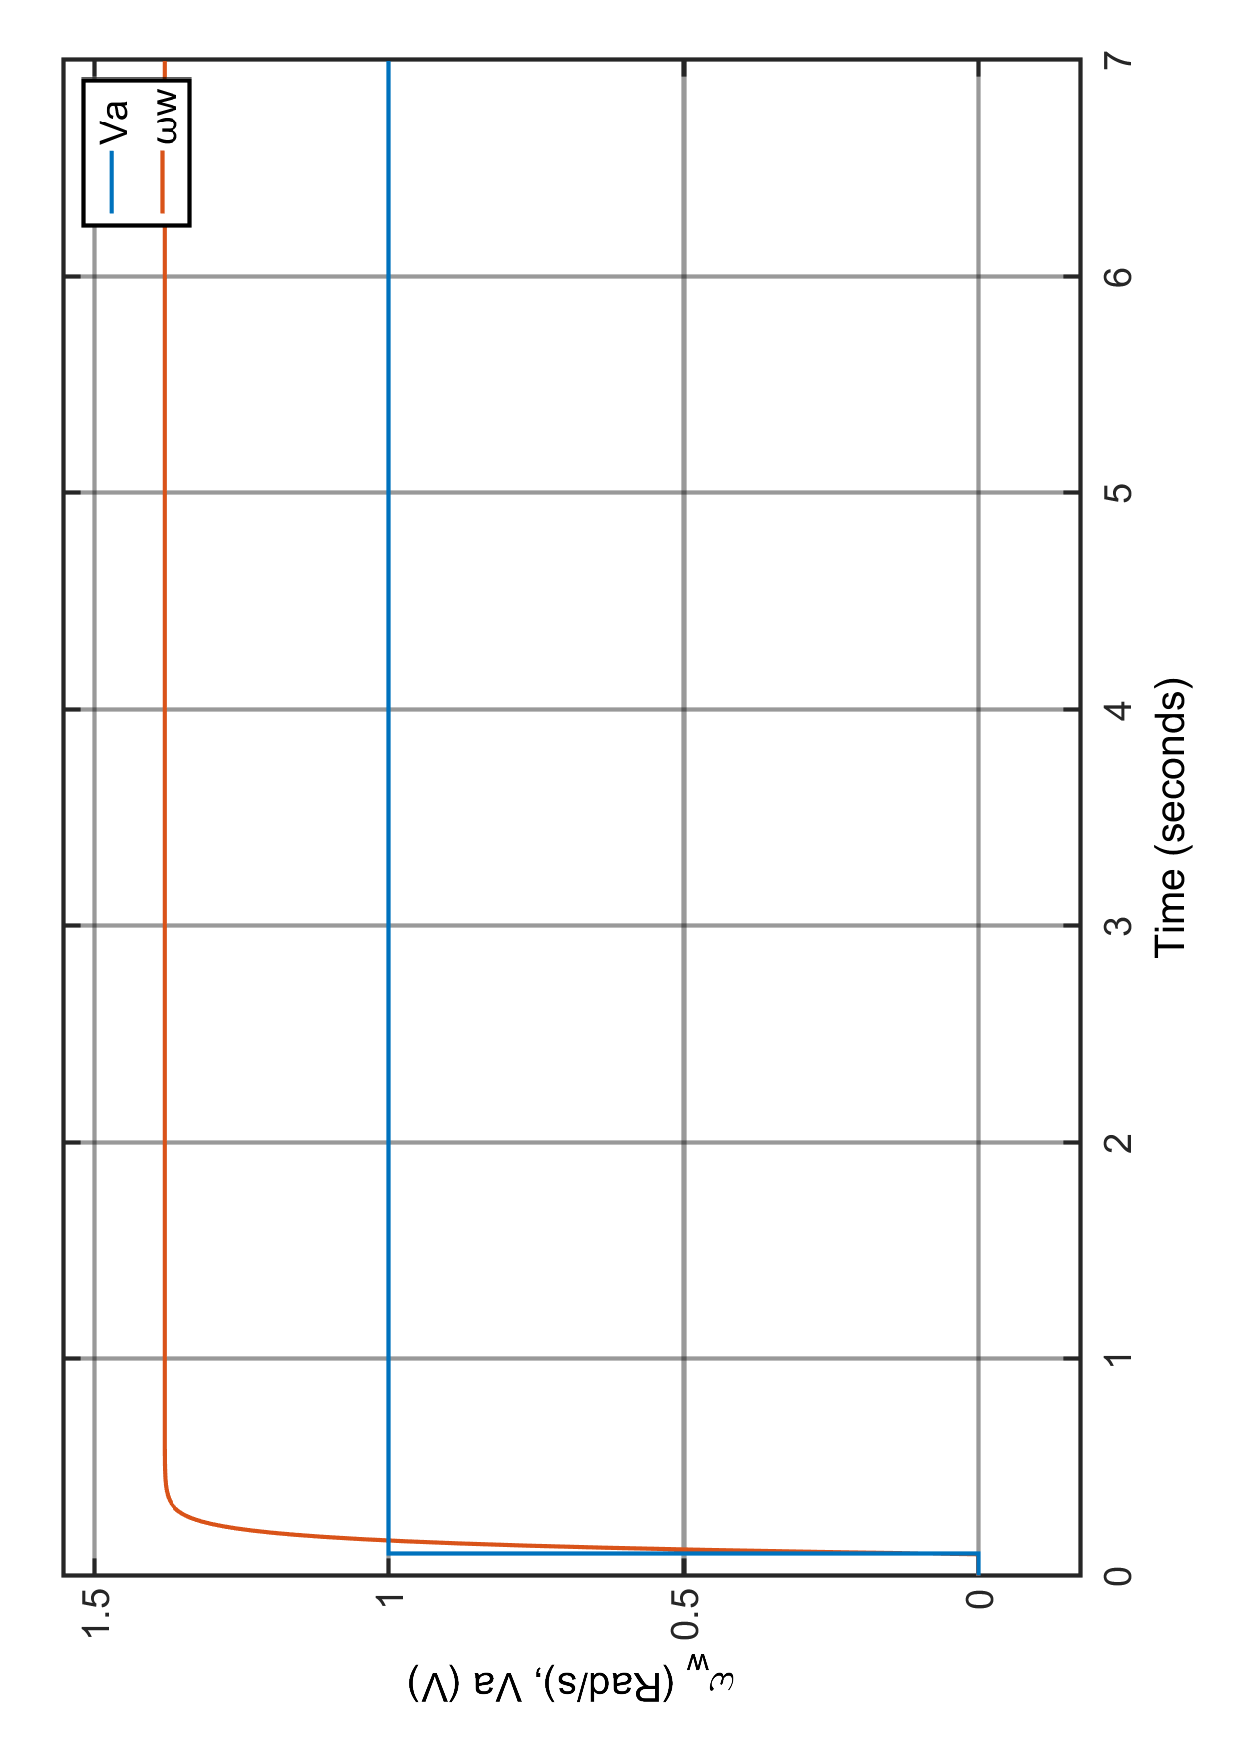
\includegraphics[height = 0.75\textwidth, angle = -90]{figures/motor1.pdf}
\caption{Simulation of motors and wheels model with an applied step as input.}
\label{fig:motor1}
\end{figure}
Looking at the expression for the motors and wheels model in \autoref{motorsAndWheels}, it is seen that the system is a first order when removing the final term in the expression. This is because the highest order of derivatives of $\omega_m(t)$ is one, giving a first order transfer function. This is partly due to the approximation done in \autoref{eq:electricMotor2} about disregarding the inductance in the motor.
From \autoref{fig:motor1}, it can be seen that the output of the motor mimics a first order system's output, as the response is approaching the reference, without any oscillation or overshoot, which is not possible for a first order system. Therefore, the output of the simulation matches what is expected, and the model is therefore assumed to be valid.

The inverted pendulum model \autoref{eq:model1W} is also simulated in Simulink. The input to this model is chosen to be $\ddot{x}_c$ since this is the input parameter in \autoref{eq:model1W}, by means of the expression $\ddot{x}_c = r_w\ddot{\theta}_w$. Also note that the inverted pendulum is initialised at an angle of -0.05 rad. The result can be seen in \autoref{fig:pend1}.
\begin{figure}[H]
\centering
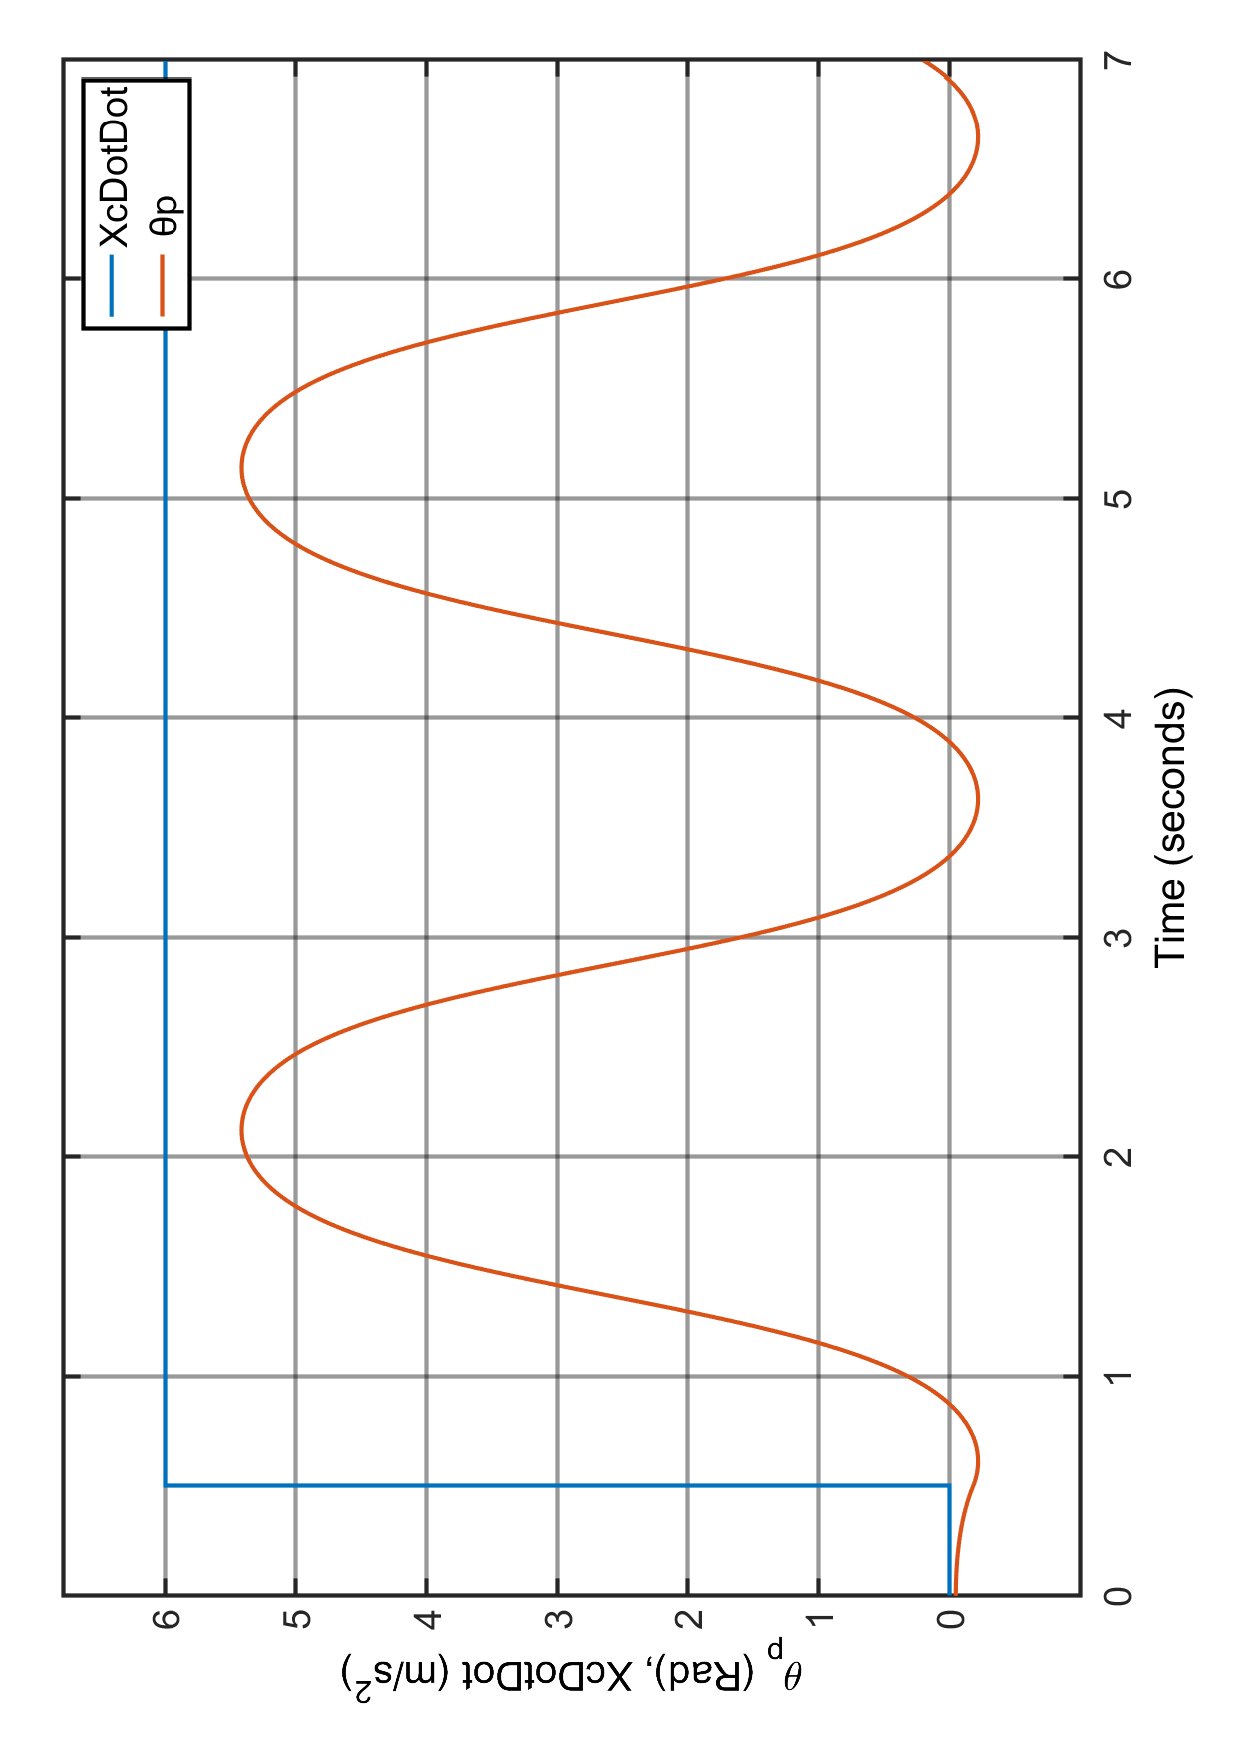
\includegraphics[height = 0.75\textwidth, angle = -90]{figures/pend1.pdf}
\caption{Simulation of the inverted pendulum model with an applied step as input.}
\label{fig:pend1}
\end{figure}

From \autoref{fig:pend1} it can be seen that the inverted pendulum starts tilting to one side, and when the step is applied, the angle changes direction and lastly the inverted pendulum oscillates around a certain angle. This angle is $\pi$ if the pendulum is swinging freely, corresponding to it hanging downwards, however an offset from $\pi$ is seen, due to the step applied. Thus, the inverted pendulum model is assumed to be valid.

To validate the system model, the motors and wheels model and the inverted pendulum model are combine and simulated in MATLAB. As an initial conditions for the simulation, the inverted pendulum is set at an angle of 1 radian, as this will cause the inverted pendulum to fall. Furthermore, a small friction is inserted in the inverted pendulum model to make the result comply more with expectations. This is done because the angle's magnitude otherwise grows, i.e. the inverted pendulum will oscillate more violently over time. This can be due to a sign error on a small number in the model. Time constraints prohibits the localisation and correction of this minor issue. The results of the simulation can be seen in \autoref{fig:systemVerification}.

\begin{figure}[H]
\centering
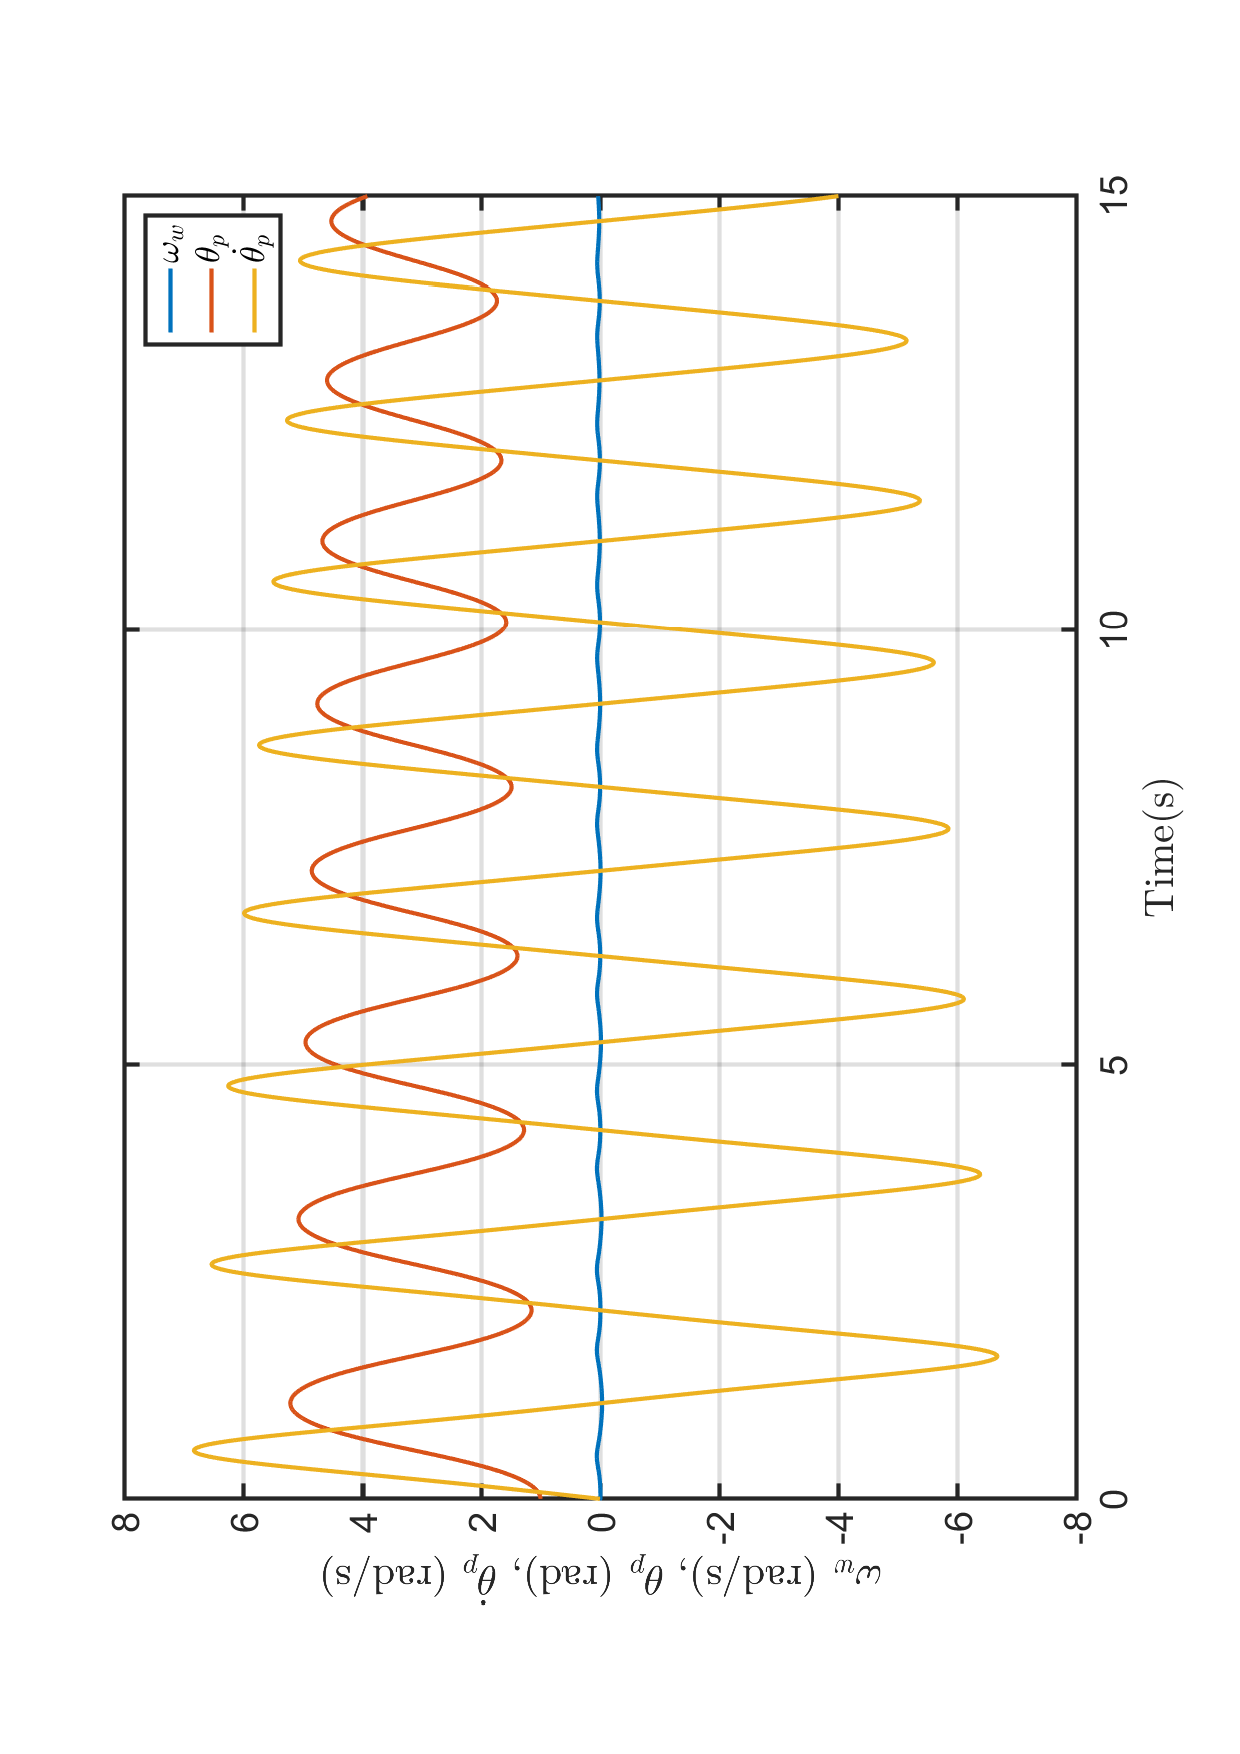
\includegraphics[height = 0.85\textwidth, angle = -90]{systemVerification.pdf}
\caption{Simulation of the system model by setting the inverted pendulum at 1 radian and no input. Note: a small friction is inserted in the model to comply more with expectations.}
\label{fig:systemVerification}
\end{figure}

From \autoref{fig:systemVerification}, it can be seen that the pendulum slowly loses magnitude due to the inserted friction. Also, it oscillates around $\pi$ which is to be expected. The model is hereby validated and can now be linearised.


\subsection{Linearisation of Derived Equations of Motion\label{subsec:Linearization}}
%In this section a transfer function describing the system is derived. This is done based on the three model equations, describing the behaviour of the segway. The transfer function is derived, so that it can be used when designing the controller. 
Before a transfer function of the system can be derived, it is necessary to linearise the two model equations, \autoref{eq:model1W} and \ref{motorsAndWheels}, as it is only linear equations that can be Laplace-transformed to form a transfer function.

It is seen that the only part of the motors and wheels model, \autoref{motorsAndWheels}, that is non-linear comes from \autoref{eq:model2W}, thus only this part needs to be linearised.
The second model equation, \autoref{eq:model1W}, also needs to be linearised as it contains non-linear terms. 

The method for doing the linearisation is chosen to be Taylor expansion.
%The last term in \autoref{motorsAndWheels} is the load torque $\tau_L$ \todo{why?}, and is approximately zero near the segway's operating point \todo{why?}. Thus \autoref{eq:motorsAndWheels} can be approximated as:
%\begin{equation}
%m_c \cdot r_w \cdot \ddot \theta_w(t) = 2 \cdot \frac{\Big(\frac{K_t}{R_A} \left( V_a(t) - K_e \cdot \frac{1}{N_{ms} N_{sw}} \cdot \dot\theta_w(t) \right) - \frac{1}{N_{ms} N_{sw}} \cdot \ddot\theta_w(t)J_{T} - \frac{1}{N_{ms} N_{sw}} \cdot \dot\theta_w(t) \cdot B_{T}\Big)}{r_w \cdot N_{ms} N_{sw}} \label{eq:model2S}
%\end{equation} 
%This approximation does not only simplify the expression considerably, but it also makes it a linear equation, as the load torque is the only nonlinear term in \autoref{eq:motorsAndWheels}.
%When approximating the load torque, it should be noted that it is only valid when the segway is at its operating point or very close to it. As the linearisation of the last model expression, \autoref{eq:model1W}, will be in the operating point as well, does not reduce the validity of the linearised model.\\
When linearising an equation, an expression for the tangent to the operating point is derived. 
% however is not alarming as the linearization of the other models, will be done in the equillibrium point as well.
%will be an approximation based on an operating point, which is in the segways equillibium position.\newpar
%The linearised model is the tangent to the chosen operating point. 
This is shown in \autoref{fig:taylor}. %This approach means that the linearised model is only an approximation of the original model around the operating point.
%During the course Modelling and control, the group was introduced to Taylor expansion as a method to linearise. For this reason the method that will be used to linearise \autoref{eq:model1W} is Taylor expansion.
\begin{figure}[H]
\centering
\input{figures/taylorFigure.ralf}
\caption{Illustration of linearisation principle.}
\label{fig:taylor}
\end{figure}

Taylor expansion is based on the Taylor series, shown in \autoref{eq:taylorSeries} \citep{sou:taylorSeries}. The Taylor series approximation of a signal is enhanced by including a greater number of terms in the Taylor series, i.e. by having an infinite sum of terms, the approximation is exact. However, since the linearisation is a tangent, only the first two terms in the Taylor series is used in the Taylor expansion, as the resulting expression is otherwise not linear.
\begin{align}
T(x) = f(a) + f'(a)(x - a) + \frac{f''(a)}{2!}(x - a)^2 + \frac{f^{(3)}(a)}{3!}(x - a)^3 + ...
\label{eq:taylorSeries}
\end{align}
\begin{where}
\begin{tabular}{p{40pt} p{42pt} p{200pt}} &$T$ & is the taylor approximation \end{tabular} \\
\begin{tabular}{p{40pt} p{42pt} p{200pt}} &$x$ & is the input \end{tabular} \\
\begin{tabular}{p{40pt} p{42pt} p{200pt}} &$f$ & is the function to be linearised \end{tabular} \\
\begin{tabular}{p{40pt} p{42pt} p{200pt}} &$a$ & is the linearisation point \end{tabular} \\
\end{where}

The linearisation is performed around the segway's operating point, which is expressed as:
\begin{equation}
\theta_p(t) = \bar{\theta}_p(t) + \hat{\theta}_p(t)
\end{equation}
\begin{where}
\va{$\theta_p(t)$}{is the angle of the inverted pendulum}{rad}\\
\va{$\bar{\theta}_p(t)$}{is the operating point}{rad}\\
\va{$\hat{\theta}_p(t)$}{is the deviation from the operating point}{rad}
\end{where}

There are three variables included in the non-linear terms in the equations that are to be linearised, i.e. $\theta_p(t)$, $\dot\theta_p(t)$ and $\ddot\theta_p(t)$. Therefore, the Taylor series has to be done for each variable, which can then be added to form the linear expression with multiple linearised variables. The Taylor expansion can be expressed as the following:
\begin{align}
T= f(\bar{\theta}_p(t),\bar{\dot \theta}_p(t), \bar{\ddot \theta}_p(t))+ \frac{\partial f(\bar{\theta}_p(t))}{\partial\theta_p(t)}\cdot \hat{\theta}_p(t)+\frac{\partial f(\bar{\dot \theta}_p(t))}{\partial \dot \theta(t)_p}\cdot \hat{\dot \theta}_p(t) &+ \frac{\partial f(\bar{\ddot \theta}_p(t))}{\partial \ddot \theta(t)_p}\cdot \hat{\ddot \theta}_p(t)\label{eq:taylor}
\end{align}

The linearisation is done in the segway's upright position $\theta_p = 0$, i.e. this is the chosen operating point.

First, the cart model, \autoref{eq:model2W}, is linearised. This is done in \appref{appTaylor}, and the result can be seen in \autoref{linGovEq2}.
\begin{equation}
(m_c + m_p) \cdot \ddot x_c(t) = F_{F}(t) + m_p \cdot l \cdot \hat{\ddot{\theta}}_p(t)\label{linGovEq2}
\end{equation}

Analysing this equation, and comparing it to \autoref{fig:systemVerification}, it is assumed that when the segway is being operated, i.e. a voltage is applied to the motors and the segway is therefore moving, the following is true:
$$ F_F(t) >> m_p \cdot l \cdot \hat{\ddot{\theta}}_p(t) $$
This means that the force applied from the motors is much bigger than the force the inverted pendulum exerts on the cart. Based on this assumption, the inverted pendulum's influence on the cart's position is neglected, i.e. the last term in \autoref{linGovEq2} is removed. In a physical sense, this would mean that when the inverted pendulum is tilting, the cart will not move. Obviously, this is not the case, but the movement caused by the inverted pendulum is much smaller than the movement caused by the motors and wheels, and it is therefore seen as a fair assumption to make. This serves to make the model simpler, by removing the feedback from the pendulum to the cart.\\
This simplified linearised expression can then be combined with \autoref{eq:model3W} and \autoref{eq:tauFFrelation}, to obtain a linear expression for the motors and wheels model, which can be seen in \autoref{eq:model2S}.
\begin{equation}
(m_c + m_p) \cdot r_w \cdot \ddot \theta_w(t) = 2 \cdot \frac{\Big(\frac{K_t}{R_a} \left( V_a(t) - \frac{K_e}{N_{ms} N_{sw}} \cdot \dot\theta_w(t) \right) - \frac{J_{T}}{N_{ms} N_{sw}} \cdot \ddot\theta_w(t) - \frac{B_{T}}{N_{ms} N_{sw}} \cdot \dot\theta_w(t) \Big)}{r_w \cdot N_{ms} N_{sw}} \label{eq:model2S}
\end{equation} 

With the motors and wheels model linearised, the inverted pendulum model shall also be linearised. The inverted pendulum model, see \autoref{eq:model1W}, is linearised in \appref{appTaylor}, which yields:
\begin{align}
(J_p+m_p\cdot l^2)\cdot \hat{\ddot \theta}_p(t) = m_p \cdot l \Big(g \cdot \hat{\theta}_p(t) + r_w \cdot \ddot \theta_w(t)   
\Big)\label{eq:firstModelLin}
\end{align}
Both model expressions are now linear and can be Laplace transformed to yield transfer functions, which is necessary to be able to design a controller for the segway. The segway's transfer function is now to be determined.
%The equation are shown in \autoref{eq:firstModel}, where each term that will be linearised by applying the Taylor expansion, shown in \autoref{eq:taylor}, is marked. The linearised approximation is shown in \autoref{eq:firstModelLin}.


